%%==================================================
%% chapter1.tex for BIT Master Thesis
%% version: 0.1
%% last update: Nov 8th, 2017
%%==================================================
\chapter{绪论}\label{chap:intro}
\section{本论文研究的目的和意义}\label{sect:1.1}

自动控制理论的进步和发展意味着动态系统的性能更优,意味着生产力的提高和自动化程度的提高等,因此自动控制在工程和科学领域一直都起着至关重要的作用。自动控制的基本思想可以追溯到公元前300年左右\upcite{CLiZhuLi2004},其理论的初步形成源于在二十世纪中叶奈奎斯特、伯德、维纳等人建立的经典控制理论,主要运用频率法和根轨迹法等分析工具;1960年左右,Kalman 等人提出的状态空间方法与概念标示着现代控制理论与方法的萌芽和诞生。而后,自动控制系统的运行环境越来越复杂,人们对系统控制的目标越来越多,要求也越来越苛刻。随着科学技术的发展和应用需求的不断催生,加上众多学者的不断努力,基于状态空间、传递函数等反馈理论基础和实践过程,现代控制理论迅速兴起。近年来,不论是在现代工业领域,还是在国防科技领域,现代控制理论都发挥着举足轻重的作用。线性系统理论、系统辨识理论、最优控制理论、自适应控制理论和鲁棒控制理论等重要分支的蓬勃发展,促进了自动控制在机器人伺服系统、工业过程、航空航天、人口与经济控制等领域的应用。

在经典控制理论和现代控制理论中,通常假设被控对象是线性系统并且模型的参数是精确已知的,然后以此为前提设计控制律。典型的控制方法\upcite{Katsuhiko2005,Pan1990}就是比例-积分-微分(PID)控制、极点配置\upcite{BraschPearson1970}、线性二次型调节器等。其中针对单变量的PID反馈控制算法应用十分广泛,到目前为止,工业过程大部分也都采用PID控制或者其改进算法。实际系统从本质上来说都是非线性的,而非线性系统的表现形式丰富多彩,比如饱和、时滞、间隙、死区等;对这些的复杂非线性系统, 目前没有很好的系统辨识方法和实际测量工具能够给出系统精确的建模结果,对系统认知的有限性和对系统模型不精确描述,造成系统普遍存在一定的不确定性;许多系统例如机器人、飞行器等运动控制系统都是强耦合的,增加了系统的不确定性。系统的非线性(nonlinearity)和不确定性(uncertainty)给分析和设计控制律带来了极大的挑战。一方面,由于系统工作环境和时间累积的影响,系统实际模型的参数和标称模型的参数总会存在不确定的误差,系统的负载和惯量也会在长时间运行之后发生变化,这些因素都导致了系统参数的不确定性,如果不加以处理可能降低系统的性能。另一方面,系统中可能存在的未建模动态、执行器的非线性特性等,也会增大系统的不稳定性和整体性能,如摩擦非线性会引起伺服系统在低速运转下的不平稳,出现时滞现象;而输入间隙、死区则容易导致系统出现抖震和极限环。因此作为影响系统控制性能的重要因素,与系统不确定性特别是非线性系统的不确定性相关理论研究和实际运用一直备受关注。

随着计算机技术、网络技术的飞速发展,越来越多的控制系统采用数字微处理器作为控制器,特别是机器人伺服系统、航空航天控制系统等运动控制领域。数字化和网络化是现代伺服电机和飞行控制器等的发展趋势。机器人和飞行器等本体作为被控对象,从本质上来说都是连续时间系统,而给这些被控对象施加的都是离散控制信号,只是采样时间很短,通常在毫秒级别。为了简化,在给这些系统设计控制律的时候,常常借助于连续时间控制理论去设计,然后直接施加离散时间控制信号。这样的手段在使用过程中一般不会出现问题,但是存在着隐患,因为系统离散化后特性常常发生变化,也就是输入输出关系发生了改变,特别是非线性和不确定性等特性经过离散化变得更加不可预测。例如,摩擦、死区等非光滑非线性经过离散化之后,更加难以用数学模型精确描述或近似,增加了系统的不确定性。如果不加考虑,可能会使得系统不稳定。因此,从离散时间角度研究实际系统的控制问题更加符合真实条件。

本文将上述的非线性、不确定性和离散化导致的未知因素统一归纳为参数不确定性(parametric uncertainty)和非参数不确定性(non-parametric uncertainty)。随着控制理论的不断发展,对非线性系统的不确定性的处理方法也越来越多,如 鲁棒控制、自适应控制等。在这些方法中,自适应控制基于其完善的理论基础和良好的鲁棒性能,在系统不确定性的相关研究中起着极其重要的作用。自适应控制在线性系统中的应用相对来说已经比较成熟,基于连续时间对象的自适应控制算法也层出不穷。然而针对同时具有参数不确定性和非参数不确定性的离散时间自适应控制相关研究还处于探索阶段。本文将借鉴一些其他领域的思想,如机器学习、数据驱动、先验信息关联、计算几何等,解决同时存在这两种不确定性的系统的控制问题,这一方向的研究具有相当大的理论意义和实用价值。

\section{国内外研究现状及发展趋势}\label{sect:1.2}
下面介绍本课题涉及到的理论和方法在国内外的研究现状和主要发展趋势。
\subsection{自适应控制}%\label{subsec:***} 可标注label

一般认为,自适应控制的相关理论和技术起源于二十世纪五十年代解决不同飞行高度飞行器的控制器设计问题。自适应控制是在指在被控对象的参数未知或者时变的情形下,在常规反馈控制器中引入自适应算法,动态地对控制方案进行调节,以抵消被控对象的模型时变或受到较大干扰的影响。线性系统的自适应控制方法已经比较成熟,在解决线性被控对象在参数未知和时变情形下取得了比较满意的控制效果。自适应控制的核心思想在于对系统不确定性进行估计、辨识和学习,同时设计出稳定的控制律,这使得控制器能满足系统的实际情况。辨识与控制的具体设计是实现自适应估计与控制哲学的关键步骤。模型参考自适应控制(Model Reference Adaptive Control, MRAC)和自校正控制(Self-tuning Control, STC)是解决线性系统的两类典型自适应控制方法。除了这两种写入教科书的经典自适应控制方法外,经过数十年的发展,针对不同特点的系统,形成了许多自适应方法,如特征模型全系数自适应控制、集值系统自适应控制、L1-自适应控制、无模型自适应控制等;另外,自适应控制思想与其他方法结合,还涌现了一系列自适应控制方法,如和PID结合形成自适应PID整定,与模糊数学结合形成模糊自适应控制\upcite{MaZhangZhou2016}等。

除了自适应控制,在解决系统的不确定性问题时,鲁棒控制也是一种比较常用的方法。当系统存在一定程度的参数不确定性和未建模动态时,鲁棒控制方法可以使得闭环系统仍能保持稳定,并保持一定的动态性能\upcite{BallCohen1987}。一般来说,鲁棒控制器的设计和最终效果都依赖于对系统不确定性程度的先验假设。为了使系统稳定,常常假设系统的不确定性在较小的范围内,并且鲁棒控制器设计过程中某些项的对消或者抑制等也严格利用了系统的假设结构和精确的先验知识,这样导致鲁棒控制不能解决系统存在较大不确定性的情形。相对于鲁棒控制,自适应控制由于在反馈回路中嵌入了在线学习机制,因此能够对付比较大的系统不确定性。

针对非线性特性或者非参数不确定性的辨识方法常常是设计出性能满意的自适应控制律的难点,特别是对于现代数字化控制器,在被控对象的数据经过离散采样化之后系统对应的结构和参数都存在较大不确定性。虽然经典的控制理论是从连续时间系统的研究出发,并且现代控制理论很多也是基于连续时间对象考虑的,但是在许多实际应用中也取得了比较好的控制效果。但是,基于模拟量的连续控制器由于扩展性和可重构性差,且设计复杂的控制规律时十分复杂,随着计算机技术的发展逐渐被历史淘汰。相反,数字化和离散化控制器越来越被广泛应用。实际的被控对象是离散时间系统,这样从连续时间角度设计的控制器嵌入到实际过程中形成闭环系统后,与理论分析有较大偏差,这必然会限制实际的控制性能的提高。

经典的模型参考自适应控制主要针对连续时间系统建立。自校正控制从一开始就是针对离散时间系统而建立的自适应控制规律,即可考虑如下被控对象
\begin{equation}%
\label{eq:1.ARX}
y_{k+1} = \bm{\theta}^{\tau}\cdot\bm{\phi}_{k} + \epsilon_{k+1}
\end{equation}
其中,$u_{k}$,$y_{k}$在$k$时刻的系统输入和输出;$\bm{\phi}_{k} = [y_{k},y_{k-1},\ldots,\y_{k-p+1},u_{k},u_{k-1},\ldots,u_{k-q}]^{T}$;$p$和$q$分别是系统输出变量$y_{k}$和输入变量$u_{k}$的阶数;$\bm{\theta}$是待估计的参数;$\epsilon_{k}$是干扰。对于\eqref{eq:1.ARX}这样的被控对象,使用最小二乘算法(Recursive Least Squares, LS)去辨识未知参数$\theta$,或者递推最小二乘算法(Recursive Least Squares, RLS)\upcite{ChenGuo1991}及其诸多变体(如加入遗忘因子的RLS\upcite{Guo1992}。在解决实际问题时,自校正控制采用参数辨识和必然等价原理设计自适应控制律,这是一种比较容易理解的思路。最小二乘算法主要针对线性系统设计,因而导致经典的基于LS的自校正调节器\upcite{GoodwinRamadge1980}难以对付强非线性的被控对象,相关对比实验也表明了从线性系统角度出发设计的自适应控制在碰到存在具有强非线性的不确定性系统时的捉襟见肘\upcite{MaLum2009}。这常常表现为系统的跟随性能满足不了要求,系统的实际输出与期望值存在较大偏差,或者系统难以对付较大的非线性干扰。不过,传统自校正控制算法设计中的必然等价原理对后续的自适应控制器的设计有很好的指导意义。

上述讨论的模型\eqref{eq:1.ARX}常常被称为带外部输入的自回归模型(auto-regression model with extra input, ARX)\upcite{ChenZhao2014},其中的未知参数向量$\bm{\theta}$刻画了系统的不确定性,但只是考虑到了参数不确定性。另一种模型被称为Nonlinear ARX(NARX)模型,其单输入单输出情形的方程为
\begin{equation}%
\label{eq:1.NARX}
y_{k+1} = f(y_{k},y_{k-1},\ldots,y_{k+1-p},u_{k},u_{k-1},\ldots,u_{k+1-q})+\epsilon_{k+1}
\end{equation}
其中,$f(\cdot)$代表某个未知的非线性函数。方程\eqref{eq:1.NARX}从非线性的角度刻画了系统的不确定性,将系统当作一个几乎可以说是黑箱的模型,几乎完全不受限于系统的具体结构和参数,直接建立系统输入输出的对应关系。除了随机干扰之外,\eqref{eq:1.NARX}整个系统的不确定性主要体现在未知函数关系$f(\cdot)$上,显然其囊括了线性过程\eqref{eq:1.ARX},似乎可以当作一种通用的模型,从而解决之前的问题。然而,要解决好系统\eqref{eq:1.NARX}的自适应控制问题十分困难,有赖于较好的非线性辨识方法和基于辨识结果设计出合适的控制输入$u_{k}$的表达式,这就涉及到非线性离散时间自适应控制,这种非线性控制方法\upcite{Li2010,Hou2006,YangDaiLee2009}也都大多针对满足一定简化条件的非线性模型或者某一特定的被控对象进行研究,针对不同的结构采用不同的方法,设计和分析都比较复杂,且通用性较差。

解决具有较大不确定性的非线性系统时,难以找到合适的参考模型与之对应以及难以满足匹配条件,就难以实施模型参考自适应控制方法。从必然等价原理出发实施自适应控制需要解决非线性系统的辨识(identification)与估计(estimate)问题。辨识高阶复杂的受控对象模型依赖于很好的辨识算法,并且,高阶复杂的系统辨识容易导致高阶复杂的控制器,而高阶复杂的控制器会给控制技术的具体实施、诊断维护、成本控制等带来一系列困难。有一些基于数据驱动的自适应控制避开了这个问题,例如,无模型自适应控制\upcite{Hou2014}依据系统的输入输出数据设计控制律,充分利用了数据驱动的思想,不过其算法依赖于动态线性化数据模型的准确性,其假设模型具有局限性。综上所述,在伺服电机、机器人、飞行器等具有强非线性、强耦合的离散时间被控系统中,未知参数、非线性动态特性、未知干扰和控制器离散时间化带来的不确定性等这些问题并得到没有很好的解决。

设计上述被控对象的自适应控制器的难点在于如何解决同时存在被控系统的参数不确定性和非参数不确定性\upcite{YangChaiZhai2009}。运动控制系统在高速或者超低速等情况下往往具有很大的不确定性,需要自适应反馈,诸如此类。近年来,郭雷院士等学者\upcite{XieGuo1999}指出自适应反馈机制是存在极限的。受自适应反馈机制的最大能力和局限这一研究方向的启发,马宏宾等学者\upcite{MaLum2009}引入基于集合的辨识方法和数据驱动的思想,归纳出了一种等价模型,即半参数系统(semi-parametric system)用来刻画大部分非线性离散时间对象,由此提出了半参数自适应控制这一研究方向。相比于前面提到的常见自适应控制算法,半参数自适应控制出发点具有独特性,和常见的自适应控制算法的详细比较见表\eqref{tab:adaptive}。半参数自适应控制这一研究方向结合了先验信息和数据驱动的思想,设计思路不依赖于具体的被控对象,是一种比较新颖的思路。目前半参数自适应控制中的非线性部分辨识主要考虑采用的是最近邻估计(nearest-neighbor estimate),这种方法未必最优,可以引入其他非线性辨识方法作进一步的优化和扩展。半参数自适应控制目前正处于探索期,还有待于深入和推广。

\begin{table}
\centering
\caption{常见自适应控制算法比较}\label{tab:adaptive}
\begin{tabular*}{0.9\textwidth}{@{\extracolsep{\fill}}cccc}
\toprule
算法名称		&主要时间特性	&适用对象	&系统不确定性类别 \\
\midrule
模型参考自适应控制		&连续时间	&线性系统&参数\\
自校正调节器		&离散时间	& 线性系统&参数\\
无模型自适应控制		&离散时间	&非线性系统&非参数\\
半参数自适应控制		&离散时间&非线性系统	&参数和非参数\\
\bottomrule
\end{tabular*}
\end{table}

\subsection{非线性估计与神经网络}%\label{subsec:***} 可标注label

通常的自适应控制主要处理在控制科学中的参数不确定性,尤其是线性参数不确定性,然而实际系统经常是参数不确定性和非参数不确定性共存,这就给实际的应用带来了很大的困难。为了实现对含有较大非线性特性的不确定被控对象的控制,常用的做法是利用系统的输入输出数据去估计系统的非参数不确定性,为设计出满足性能要求的控制律提供依据。从数学上看,自适应控制中的辨识与估计类似于机器学习(machine learning, ML)\upcite{Anonymous2014},两者的交叉点在于都是通过数据修正输入输出映射关系这一过程来改善系统的性能。基于数据驱动的机器学习方法以客观存在的事物为对象,研究数据的客观规律,实现数据的分类和预测。机器学习是人工智能的核心\upcite{ZhouML2016},是使计算机具有智能的根本途径。自从上世纪中叶以来,机器学习在理论研究、算法设计和工程应用等方面都取得了飞速发展。

人工神经网络(Artifical Neural Network,ANN)是机器学习的一个庞大的分支,通常用于解决分类和回归问题。20世纪感知机和神经网络概念被提出以来,有关神经网络((Neural Network,NN))的研究走过的是一条波浪式推进、起伏跌宕的发展道路,其在模式识别、不同的领域应用已经十分广泛[23]。神经网络的基本结构示意图如图\ref{fig:MNN}所示,主要包括1个输入层、0个或多个隐含层和一个输出层。

\begin{figure}
 \centering
 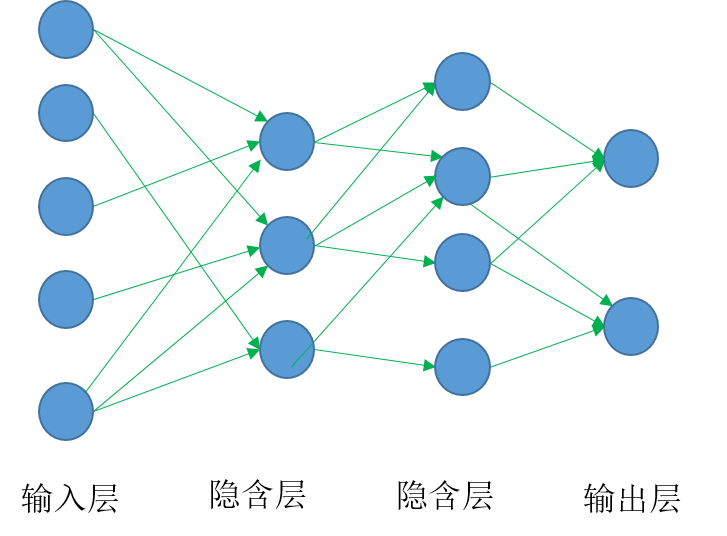
\includegraphics[width=0.55\textwidth]{ch1-NN.png}
 \caption{多层前馈神经网络的结构示意图(含2个隐含层)}\label{fig:MNN}
\end{figure}

一般认为,网络结构、激活函数(activation function)和学习算法是神经网络的三大要素。神经网络的分类主要依据这三要素,而学习能力是其主要特点\upcite{HanXieFu2014}。学习过程是根据训练数据,通过不断修正神经元之间的连接权值及每个神经元的阈值来实现的。它对非线性系统和难以直接建模的系统具有良好的效果。人工神经网络的模型按照信息的传递方向,通常可以分为前馈型神经网络和反馈型神经网络等。在实际的控制系统应用中,由于反馈神经网络运算十分耗时间且设计复杂,因此对于在线动力学辨识和实时控制系统应用较少。前馈结构在解决高度非线性和严重不确定性系统的建模与控制方面具有很大潜力。将神经网络引入控制系统是重要的突破\upcite{NarendraKannan1990},陆续出现了神经网络逆控制、神经广义预测控制、自适应神经输出反馈控制和模糊神经网络控制等方法。

对于控制界,神经网络的吸引力在于其强大的非线性建模与辨识能力,主要体现在以下几个方面:
\begin{enumerate}
\item 逼近能力。神经网络能够逼近任何一个非线性函数,因而能以非常高的精度逼近具有复杂动态特性的非线性系统;
\item 容错能力。一般神经网络都存在大量神经元,类似与动物的神经中枢系统,网络中少数神经元的连接损坏几乎不会影响系统的整体功能,因而表现出很强的鲁棒性和容错性;
\item 并行计算。同一层神经元的更新计算几乎可以同步进行,因而容易部署成并行分布处理的结构,这大大提高了实时性。
\end{enumerate}

不过,神经网络的巨大优势,也难以掩盖其在解决实际控制领域应用时存在的诸多问题。例如,尽管研究出了很多神经控制算法,但绝大多数难以进行有效的闭环系统稳定性分析;神经网络的训练依赖于大量数据,而实际控制系统在很多情况下只能提供小样本量的数据,针对被控对象特性在不断变化的情形,一些传统神经控制就难以满足性能要求;快速在线学习是实时控制算法的关键,而目前大部分神经网络采用基于梯度的学习算法(如误差反向传播,Back Propagation,简称BP),计算量十分耗时。综合这几方面的因素,研究和开发新型神经网络,以及相应的实时学习算法,并将其用于控制系统中,已经成为是基于神经网络的自适应算法研究的重要方向。

\subsection{超限学习机与控制}

如前所述,目前的神经网络结构和学习算法难以满足控制系统的实时性、准确性等要求。传统的神经网络需要人为设置大量的网络参数;在网络训练时主要采用BP算法,需要耗费很长的时间多次迭代才能修正权值和隐元的偏置\upcite{ZhuHouXiong2005};由于使用梯度下降有陷入局部极小的缺陷,而未到达全局最小。一些研究学者也开始研究基于神经网络的实时辨识与控制算法\upcite{KorjaniBazzaz2008},但针对的是特定的问题,难以做到通用性。

2004年,黄广斌等人针对单隐层前馈神经网络提出了一种新颖\upcite{HuangZhuSiew2004,HangSiew2005}的学习算法,即超限学习机(Extreme Learning Machine, ELM)。超限学习机(最早有时称为极限学习机)的实现过程\upcite{HuangZhuSiew2006}主要分为三个阶段,首先初始化输入权重和隐含层神经元的偏置,然后根据输入计算出隐含层的输出,最后由期望的范数解确定输出权重,一般采用欧几里得范数,类似于采用最小二乘法确定。由此看出,基本的超限学习机算法在设置好神经网络隐含层节点个数之后,算法执行过程或者称为网络学习过程中,一般不再需要调整从输入到隐含层的权重以及隐层神经元的偏置,就能直接产生最优解,因此具有学习速度快且泛化性能好的优点。这也是其名字来源的主要原因。相对于传统网络,ELM在保证更好的泛化性的同时,具有极快的学习速度,且经过改进,可以有效减少传统梯度算法常有的局部极小、学习时间长、性能指标难以保证最优等问题,对于解决许多常见的非线性问题表现出很大的应用潜力。

如上所属,超限学习机是一种通用性很强、快速准确的前馈神经网络学习算法,对于解决手写识别、目标跟踪等领域\upcite{HangHang2015}的问题取得了丰硕的成果。ELM具有很好的系统辨识能力,在控制领域也出现了不少应用\upcite{RongZhao2013},特别是在线序列版本的超限学习机(Online-sequential ELM,OS-ELM)\upcite{LiangHuang2006}及其相关变体\upcite{YangZhang2012,ShaoMeng2016},很适合解决具有强非线性的不确定性系统的在线辨识与实时控制问题,如机器人、无人车等运动控制场景\upcite{LiNai2015,WangSunMeng2016},与自适应控制理论结合,也将形成很多解决问题的思路。

\section{本文主要研究内容}\label{sect:1.3}

本文的主要研究对象是同时具有参数不确定性和非参数不确定性的离散时间系统,结合超限学习机对现有的半参数自适应控制进行扩展和改进。主要体现在:(1)系统地归纳和总结了反馈控制和自适应控制的发展历程和发展趋势,介绍了人工神经网络等重要的非线性建模方法,对现代不确定性被控系统中的控制难点进行了提炼;(2)针对同时具有参数和非参数两种不确定性的系统进行了分析,概括出了一种半参数建模方法,列举了系统常见的先验信息的数学描述;(3)针对半参数系统介绍了信息浓缩估计思想,并设计了典型情形下的具体实现算法;(4)分析了经典神经网络学习算法在自适应估计与控制应用中的优缺点,并将超限学习机引入到半参数系统的非参数部分的估计中,设计了基于超限学习机的半参数自适应控制算法;(5)将基于信息浓缩估计和超限学习机的半参数建模与控制方法应用到机器人运动控制场景中,有效地提高了伺服电机的控制性能,这是半参数控制解决实际应用的初步尝试。

本文的章节安排如下:

第一章是绪论部分,主要阐述了非线性自适应控制的研究背景和意义,总结了经典自适应控制方法的发展历程、特点与方法和存在的问题等,分析了神经网络应用于自适应估计与控制的前景和挑战,并介绍了一些快速有效的非线性辨识方法。

第二章,介绍半参数系统与信息浓缩估计算法。在反馈能力极限等前沿问题基础上,对半参数自适应思想的来源作进一步阐述,正式描述了半参数系统的数学模型,详细介绍了信息浓缩估计的思想和具体实施方法,对原有的一阶半参数自适应估计进行了扩展。

第三章,二维参数的信息浓缩估计算法设计。描述了二维参数情形下,信息浓缩估计算法的主要步骤和基本问题,并对信息浓缩变换中直线和多边形的几何关系进行了详细地分析,同时设计了信息浓缩变换的算法流程,并在数值仿真实例中验证本章设计的信息浓缩估计算法,最后讨论了信息浓缩估计的相关优化问题和主要优缺点。

第四章,离散时间半参数自适应控制。给出了离散时间情形下半参数自适应估计与控制的数学描述,用超限学习机变体算法设计了非参数部分的估计算法,同时针对半参数系统轨迹跟踪问题设计自适应控制器,并用仿真实例对比测试和验证半参数自适应控制算法的性能。

第五章,半参数自适应运动控制。分析了机器人轨迹跟踪和伺服电机运动控制中多种不确定性存在的难点,采用半参数分析方法对单轴伺服电机进行了建模,设计了基于超限学习机的半参数自适应估计与控制算法,并结合具体对象进行了仿真对比测试,从而验证估计与控制的性能。
